\begin{figure}[htbp]
\section*{ MAPK8IP3}
\centering
\begin{subfigure}[b]{0.95\textwidth}
\centering
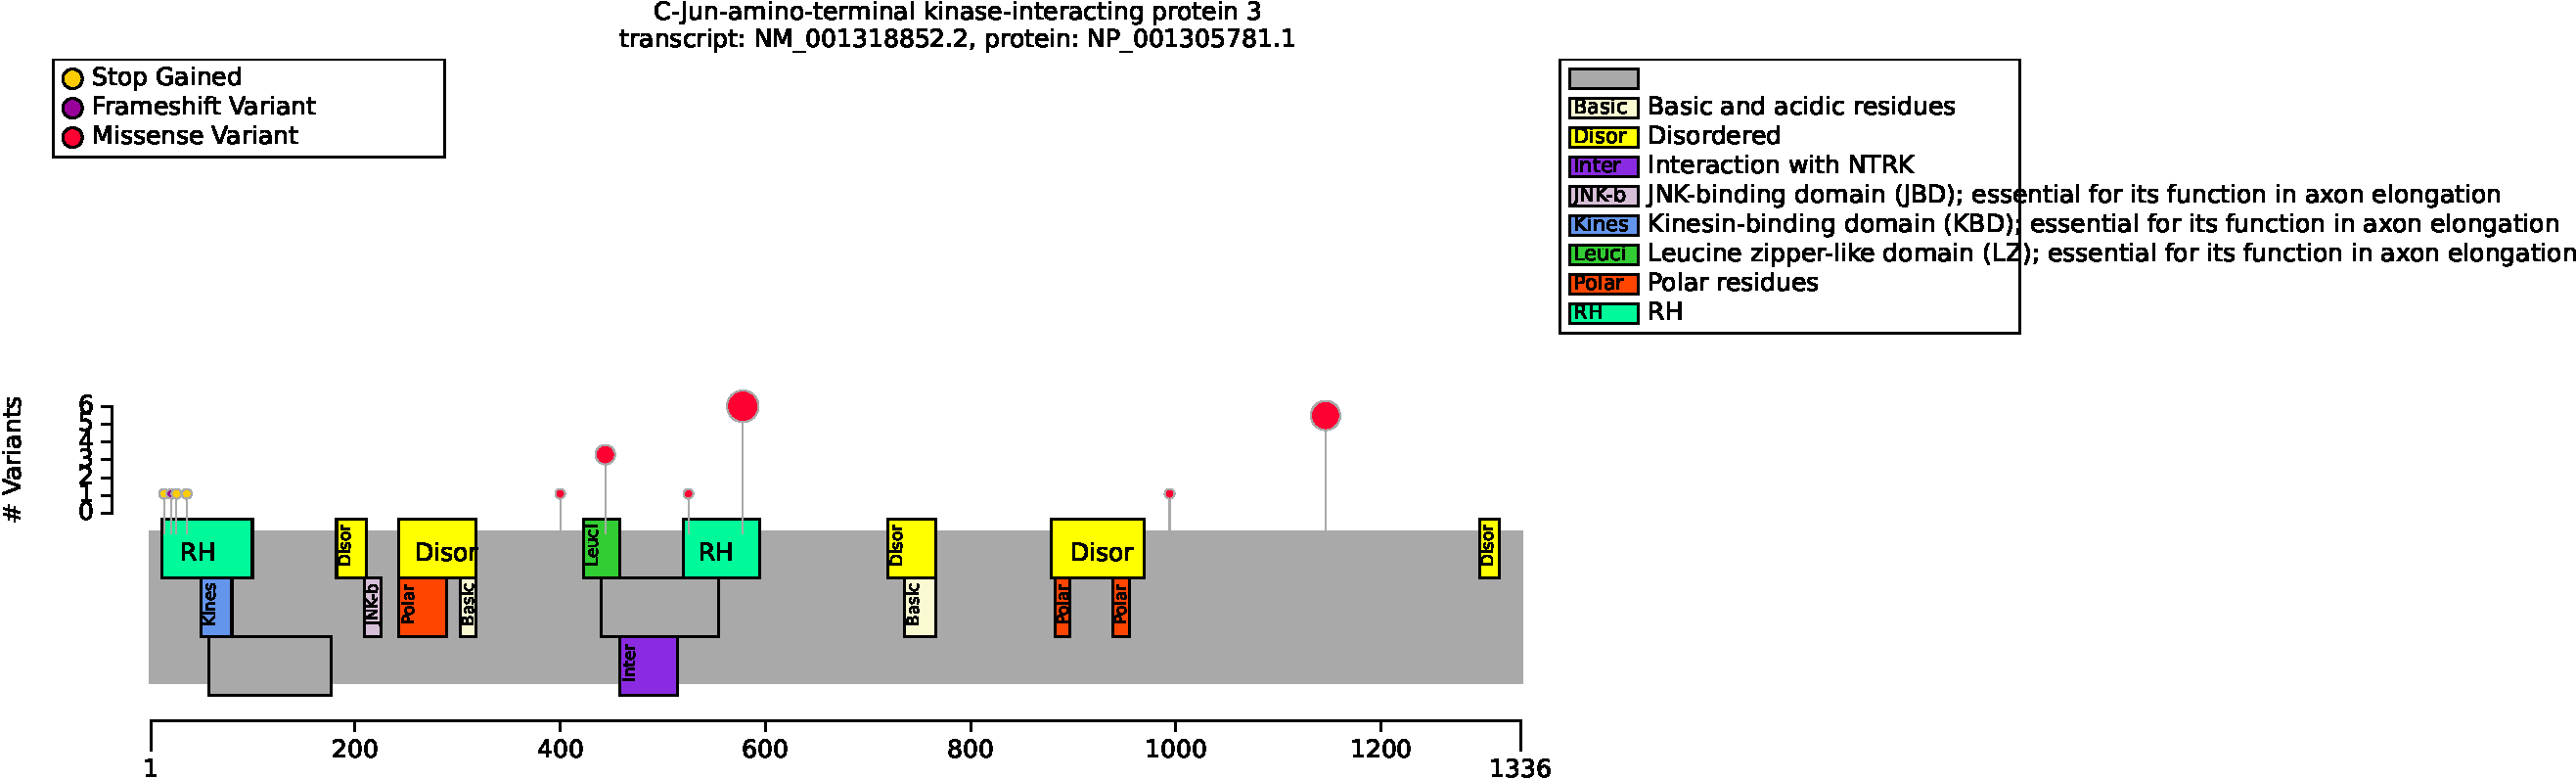
\includegraphics[width=\textwidth]{ img/MAPK8IP3_protein_diagram.pdf} 
\captionsetup{justification=raggedright,singlelinecheck=false}
\caption{Distribution of variants in MAPK8IP3}
\end{subfigure}

\vspace{2em}

\begin{subfigure}[b]{0.95\textwidth}
\centering
\resizebox{\textwidth}{!}{
\begin{tabular}{llllrr}
\toprule
Genotype (A) & Genotype (B) & total tests performed & significant results\\
\midrule
N term & other & 68 & 0\\
p.Arg579Cys & Other variant & 68 & 0\\
RH2 & Other region & 68 & 0\\
FEMALE & MALE & 68 & 0\\
\bottomrule
\end{tabular}
}
\captionsetup{justification=raggedright,singlelinecheck=false}
\caption{             Fisher Exact Test performed to compare HPO annotation frequency with respect to genotypes. }
\end{subfigure}

\vspace{2em}

\caption{ The cohort comprised 20 individuals (9 females, 11 males). A total of 93 HPO terms were used to annotate the cohort. Disease diagnosis: Neurodevelopmental disorder with or without variable brain abnormalities (OMIM:618443). No significant association identified. A total of 10 unique variant alleles were found in \textit{MAPK8IP3} (transcript: \texttt{NM\_001318852.2}, protein id: \texttt{NP\_001305781.1}).}
\end{figure}
